
\chapwithtoc{Introduction}

In today's era of information explosion and constant flow of information, it becomes more time-consuming to keep track of associations and deeply understand the published content through media and online news, primarily when investing in a specific area. For instance, the investment in a company like Apple~Inc. requires acquiring and processing a wide range of available information with significant effort and dedication in studying articles and other sources. At the same time, publicly available information resources such as news articles and tools like sentiment analysis allow us to transfer real-world context into the digital environment and use it for our benefit.

Sentiment analysis, the ability to identify and evaluate the emotional charge of content, has evolved into a crucial instrument for comprehending opinions and the general atmosphere surrounding various topics. This work focuses on developing an application that allows users to visualise connections between companies and news articles using a graph network and the impact of news sentiment on~a company's stock price.

Many experiments are currently being conducted based on historical data to examine the effect of sentiment, with promising results on datasets. The absence of such an application motivates this thesis. An application that extracts actual data from news for sentiment analysis and subsequently provides this information as an indicator of the future possible influence of a company's stock price.

One potential reason for the absence of such an application may be working with a constant flow of updating data, which can present a challenge to creating a functional application. Due to the valuable nature of news sources as information providers, they protect their data against similar usage. Despite the public availability of this data, legal complications may arise from potential violations of terms and conditions, as presented in the OpenAI, Microsoft and The New York Times dispute outlined in Chapter \ref{chap:textual-data}.

Another reason is that this is still an experimental technology and a speculative approach to the market. These technologies are still evolving, and there is no clear-cut approach to $100\%$ stock price prediction depending on news. Nevertheless, published studies involving experiments suggest correlations impact between stock prices and news data. Another notable aspect is shown in Figure \ref{fig:apple-intro}, indicating the correlation between the number of news mentioning a company and its market price. Although it may be less than $100\%$ accurate in prediction, it is an exciting topic that can be very useful for examining the impact on prices and providing an overview of the situation.
 
\begin{figure}[htbp]
    \centering
    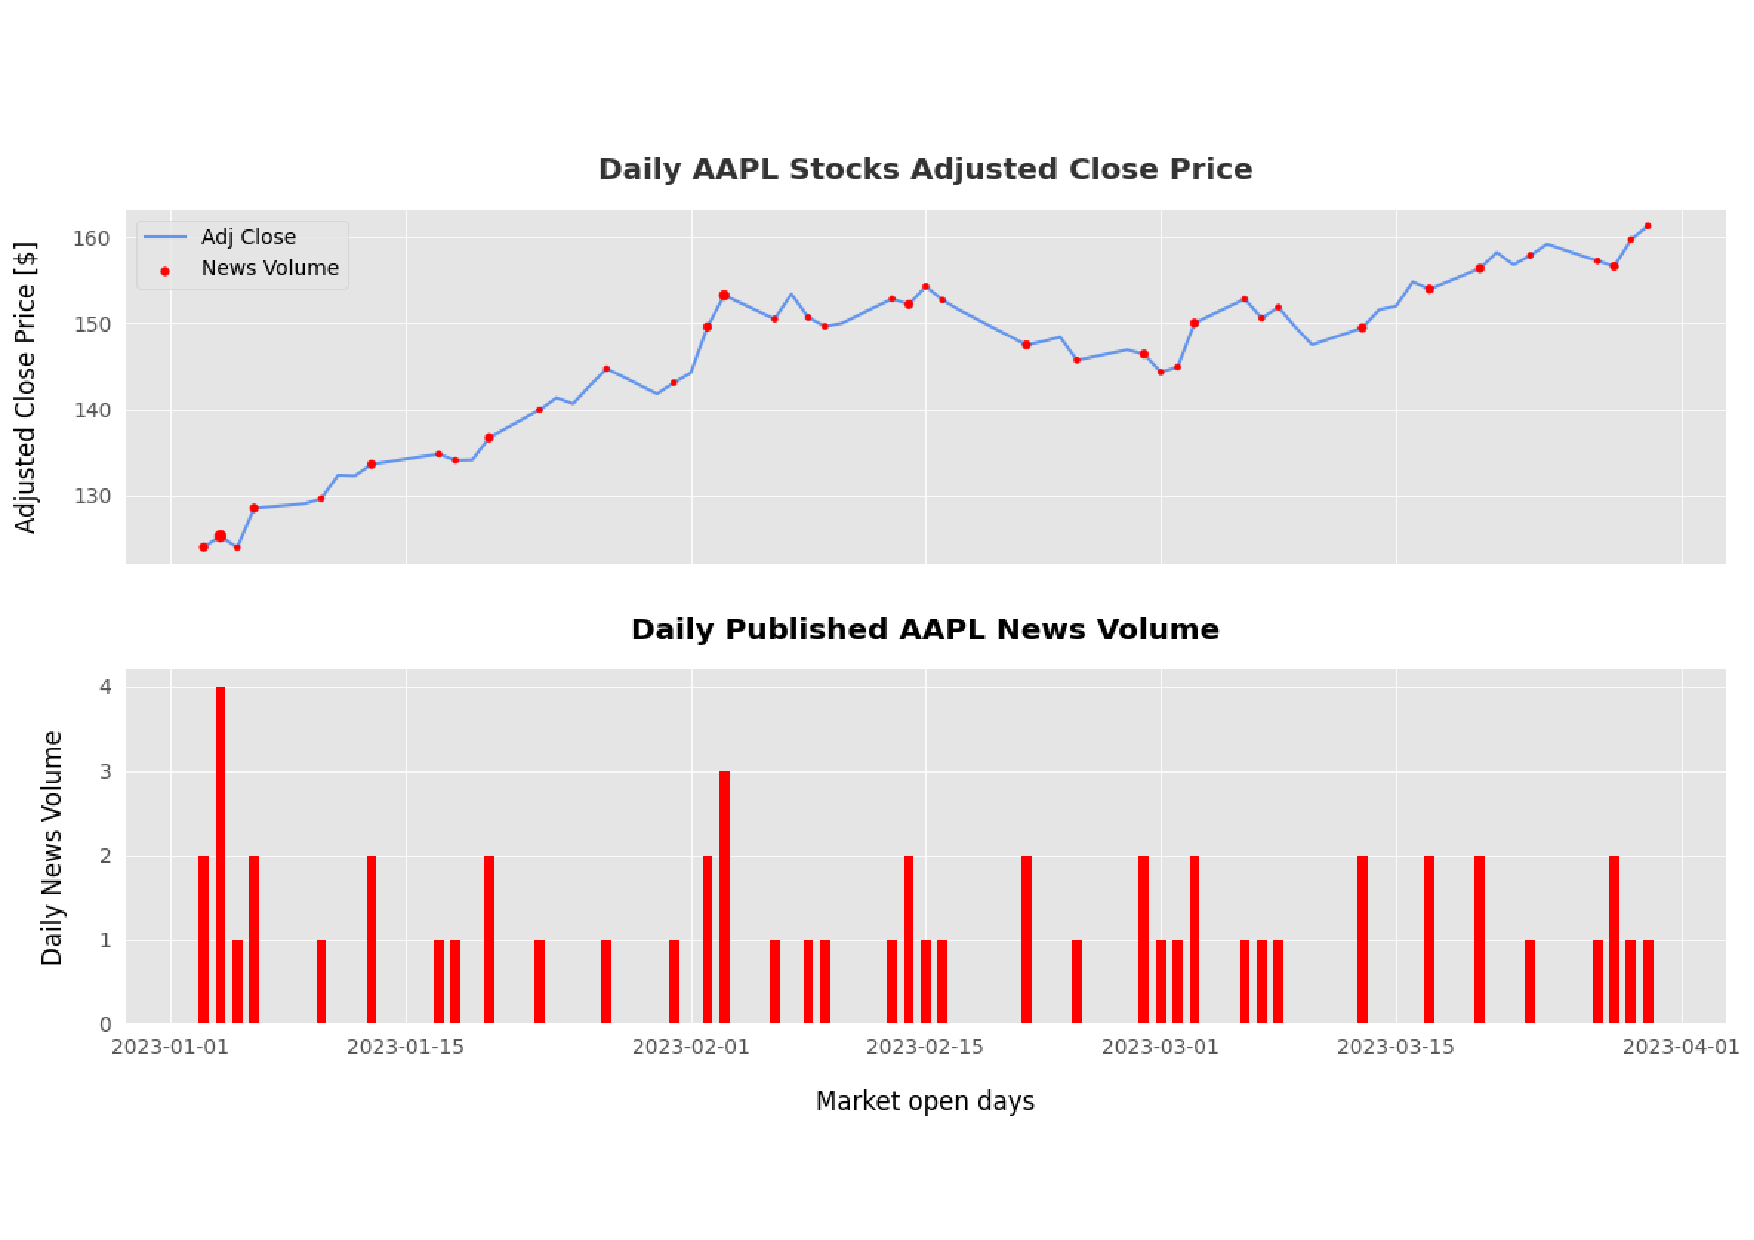
\includegraphics[width=\textwidth]{img/intro/apple-intro-a.pdf}
    \caption{Apple Inc. (AAPL) adjusted close price and the volume of news mentions in the Guardian's business and technology section in the first quarter of 2023.}
    \label{fig:apple-intro}
\end{figure}

Providing users with high-quality and reliable data is essential. Therefore, we will source data from trusted and verified newspapers and data providers. Additionally, we need to develop our algorithm for processing all data in the pipeline from extraction to recognition entity, analysis of sentiment, and loading to the database, considering there are few applications of this type, especially those focusing on entities, which is the ideal choice in our context.

The thesis is structured as follows: Chapter \ref{chap:theoretical-background} discusses the foundational concepts of sentiment analysis and named entity recognition. In Chapter \ref{chap:related-work}, we review existing applications and their methodologies in sentiment analysis, as well as recent studies related to sentiment analysis at the entity level and stock market behavior. Challenges associated with obtaining data from newspaper sources are addressed in Chapter \ref{chap:textual-data}, while Chapter \ref{chap:comapny-to-symbol-linking} focuses on detecting entities in text and extracting company names with their ticker symbols. In Chapter \ref{chap:entity-level-sentiment-analysis}, we develop an algorithm for entity-level sentiment analysis of the extracted entities and explore how this information can be used for market analysis. After describing the non-functional and functional application requirements in Chapter \ref{chap:application-requirements}, Chapter \ref{chap:architecture} covers the application architecture based on the previous chapters. We present the developer documentation in Chapter \ref{chap:development-documentation}. Chapter \ref{chap:user-documentation} is dedicated to the user documentation. Finally, the conclusion summarizes the results and discusses potential improvements and future application development.